

%%% use twocolumn and 10pt options with the asme2ej format
\documentclass[twocolumn,11pt]{asme2ej}
\usepackage[backend=biber,style=numeric,autocite=inline, sorting=none]{biblatex}
\addbibresource{bibli.bib}
\usepackage{graphicx}
\usepackage{amssymb}
\usepackage{url}

%% The class has several options
%  onecolumn/twocolumn - format for one or two columns per page
%  10pt/11pt/12pt - use 10, 11, or 12 point font
%  oneside/twoside - format for oneside/twosided printing
%  final/draft - format for final/draft copy
%  cleanfoot - take out copyright info in footer leave page number
%  cleanhead - take out the conference banner on the title page
%  titlepage/notitlepage - put in titlepage or leave out titlepage
%  
%% The default is oneside, onecolumn, 10pt, final


\title{Studying the Z Boson with the ATLAS Detector at the LHC\\
\large Advanced Lab Experiment (19th to 20th February 2019)}
\date{\today}
%%% first author
\author{Hanno I. Hennighausen
    \affiliation{
	BSc student, Heidelberg University
    }	
}

%%% second author
%%% remove the following entry for single author papers
%%% add more entries for additional authors
\author{Maximilian Rupprecht
    \affiliation{ BSc student, Heidelberg University
    }
}



\begin{document}

\maketitle    
\setcounter{page}{1}
%%%%%%%%%%%%%%%%%%%%%%%%%%%%%%%%%%%%%%%%%%%%%%%%%%%%%%%%%%%%%%%%%%%%%%
\begin{abstract}
{\it abstract
}
\end{abstract}

%%%%%%%%%%%%%%%%%%%%%%%%%%%%%%%%%%%%%%%%%%%%%%%%%%%%%%%%%%%%%%%%%%%%%%
%\begin{nomenclature}
%\entry{A}{You may include nomenclature here.}
%\end{nomenclature}

%%%%%%%%%%%%%%%%%%%%%%%%%%%%%%%%%%%%%%%%%%%%%%%%%%%%%%%%%%%%%%%%%%%%%%
\section{Theoretical background}

This section contains the minimum of needed quantities and relations. 

%%%%%%%%%%%%%%%%%%%%%%%%%%%%%%%%%%%%%%%%%%%%%%%%%%%%%%%%%%%%%%%%%%%%%%
\section{Data analysis}
In figure 
%%%%%%%%%%%%%%%%%%%%%%%%%%%%%%%%%%%%%%%%%%%%%%%%%%%%%%%%%%%%%%%%%%%%%%


\section{asdf}
%%%%%%%%%%%%%%%% begin figure %%%%%%%%%%%%%%%%%%%
\begin{figure}[h]
	\begin{center}
		\setlength{\unitlength}{0.012500in}%
		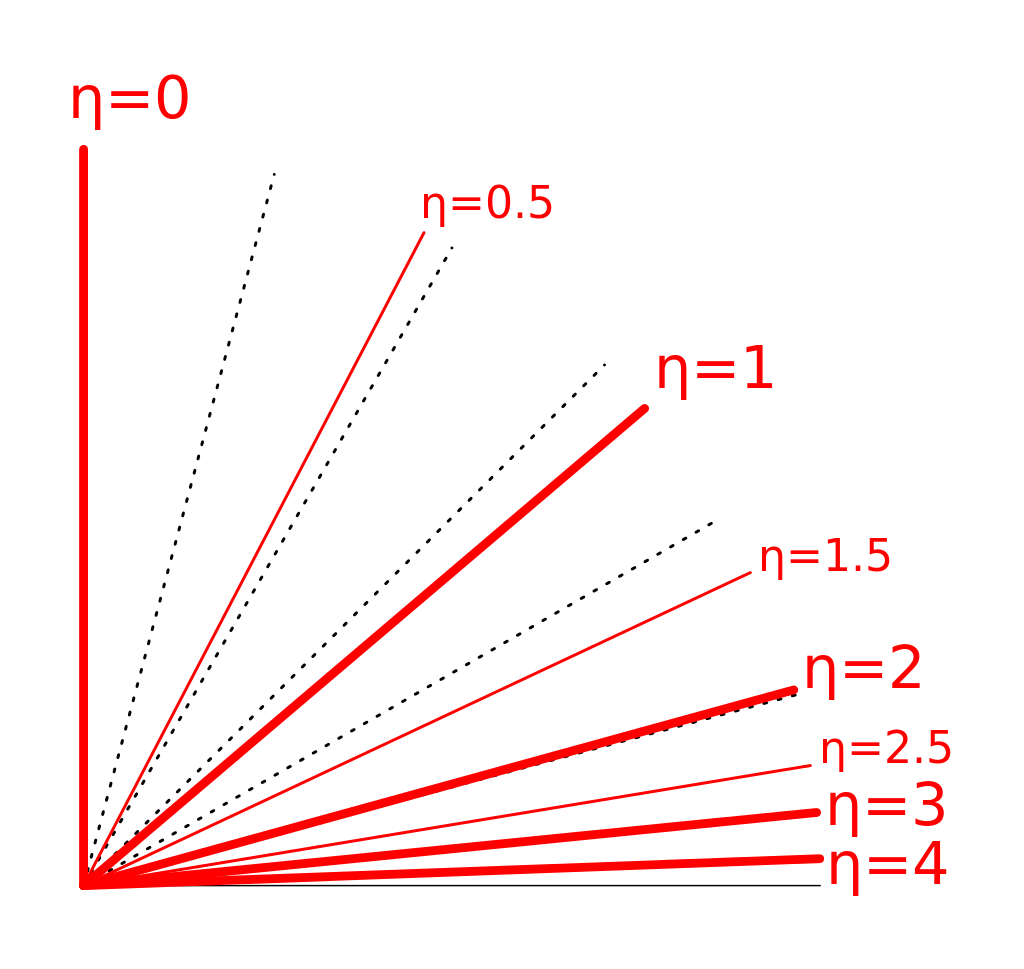
\includegraphics[width=\linewidth]{figures/pseudorapidity}
	\end{center}
\caption{Pseudorapidity}
\label{Pseudorapidity} 
\end{figure}

\begin{acknowledgment}
asdf
\end{acknowledgment}

%%%%%%%%%%%%%%%%%%%%%%%%%%%%%%%%%%%%%%%%%%%%%%%%%%%%%%%%%%%%%%%%%%%%%%
\printbibliography

%%%%%%%%%%%%%%%%%%%%%%%%%%%%%%%%%%%%%%%%%%%%%%%%%%%%%%%%%%%%%%%%%%%%%%
%\appendix       %%% starting appendix
%\section*{Appendix A: Head of First Appendix}
%Avoid Appendices if possible.


\end{document}
